\section{Introduction}\label{sec:intro}

\subsection{Background}

Digital credentials are increasingly used to verify educational achievements, professional qualifications, and trust relationships in online services. Several recent incidents point to a credibility crisis in the educational-credential space: a private university in India reportedly sold roughly $36{,}000$ fake degrees, large-scale document-forgery operations have led to student deportations, and the LinkedIn breach of 2021 exposed approximately $700$ million user profiles to the dark web~\cite{10.1007/978-981-96-0957-4_3}. Together with the rise of micro-credentials, which produce fragmented records of learning across institutions and platforms, these incidents motivate a credential system that is simultaneously \emph{verifiable}, \emph{privacy-preserving}, and \emph{long-lived}.

A long-lived credential system must satisfy two further constraints. First, it must remain secure against adversaries equipped with large-scale quantum computers; this rules out classical anonymous-credential constructions whose security reduces to the discrete-logarithm or RSA assumption. Second, it must remain practically deployable as the surrounding cryptographic and policy environment evolves: the underlying signature scheme may be updated as standards mature, security parameters may need retuning, and disclosure policies may change as institutional rules evolve. A credential system that satisfies the first constraint but is brittle under the second is unsuitable for real-world deployment.

\subsection{The Current State of Post-Quantum Anonymous Credentials}

Two representative lines of work have attempted to construct post-quantum anonymous-credential systems (the broader lattice-native and PQ-token literature is surveyed in Section~\ref{sec:related}). The first follows the lattice-based approach exemplified by Jeudy et al.\ at Crypto~2023~\cite{jeudy2023lattice}, leveraging the hardness of the Short Integer Solution (SIS) and Learning With Errors (LWE) problems. While this approach achieves quantum resistance, it currently supports only a single message per credential and yields large proof and key sizes that make repeated showings cumbersome.

The second line of work, exemplified by the recent Blockchain-based Digital Education Credential (BDEC) framework of Li, Zhang et al.~\cite{10.1007/978-981-96-0957-4_3}, takes a symmetric-primitive-based approach. BDEC instantiates a generic anonymous-credential construction with the Loquat post-quantum signature scheme~\cite{cryptoeprint:2024/868}, whose verification predicate is comparatively cheap to encode in rank-1 constraint systems (R1CS), and the Aurora transparent zkSNARK~\cite{cryptoeprint:2018/828}, which proves the R1CS relation in zero-knowledge. The resulting system achieves unforgeability, anonymity, unlinkability, conditional linkability, and revocability, and, per the authors' analysis, outperforms the lattice-based approach~\cite{10.1007/978-981-96-0957-4_3}.

A more recent post-quantum signature, PLUM~\cite{10.1007/978-981-95-2961-2_6}, is a successor to Loquat that replaces the Legendre PRF with a $t$-th power residue PRF and the FRI low-degree test with the STIR protocol. At the 128-bit security level, PLUM signatures are approximately $1.5\times$ smaller than Loquat's, and PLUM verification is expected to be up to $4\times$ faster, while requiring roughly $1.28\times$ fewer R1CS constraints~\cite{10.1007/978-981-95-2961-2_6}. Because PLUM shares Loquat's overall structure, a symmetric-primitive PRF assumption verified through a transparent low-degree test, while reporting lower verification cost at matching security, it is the signature primitive we adopt for the zkVM instantiation studied in this thesis. PLUM is a research signature, not yet standardised, chosen for its SNARK-friendly verification structure. The NIST post-quantum signature standards (ML-DSA, SLH-DSA, FN-DSA) remain the deployment baselines. Their lattice and hash verification predicates are precisely the ones that are expensive to arithmetise, and that is why a symmetric-primitive design is studied here.

\subsection{The Hidden Cost: Cryptographic Rigidity}

Both Loquat and PLUM are designed to be efficiently verifiable inside a zkSNARK. The dominant zkSNARK choice for BDEC-style constructions is a relation-specific transparent argument such as Aurora, in which the verification predicate is compiled into a fixed R1CS at deployment time. This compilation is what makes the resulting system efficient: the proof system can be specialised to the precise structure of the verification predicate.

Specialisation has a deployment-lifecycle cost that is rarely measured. Any change to the verification \emph{relation}, whether substituting the signature scheme (Loquat~$\to$~PLUM, or a future~$\Sig^\prime$), retuning a security parameter, changing the presentation \emph{structure} (the number of credentials shown, or the set of disclosed attributes), or evolving the on-chain ledger schema, requires recompilation of the R1CS matrices and re-derivation of any parameters that depend on the constraint count. (A presentation \emph{policy} that only changes which condition the verifier checks on the disclosed attributes, at fixed structure, is handled verifier-side and forces no recompilation.) In a real-world deployment that must respond to evolving NIST standardisation choices, evolving institutional policies, and evolving threat models, this cost is incurred repeatedly. We refer to this hidden cost as the \emph{cryptographic rigidity} of the static-circuit approach, and we refer to its quantitative manifestation as \emph{update churn}.

Update churn is a structural property of the relation-specific design, the price paid for specialisation, and it is the part of the cost ledger that the current evaluation literature on PQ anonymous credentials does not capture. As long as it remains uncharacterised, the deployment-cost picture of static-circuit PQ anon-credentials is incomplete: the per-change recompile wall-clock turns out to be small (Section~\ref{ssec:churn-eval}), but the regeneration-and-re-audit footprint it forces is not, and that footprint is what goes unmeasured.

\subsection{Zero-Knowledge Virtual Machines as a Structural Alternative}

A zero-knowledge virtual machine (zkVM) is a zkSNARK whose underlying relation is fixed once, at design time of the prover, to the correctness of executing a program on a deterministic instruction-set architecture~\cite{cryptoeprint:2023/1032,bruestle2023risczero,lavin2024surveyapplicationszeroknowledgeproofs}. Anything that a developer can express in a high-level language becomes a guest program; the proof system is universal. Updating the verification predicate becomes a guest-program edit under a fixed universal relation. The audit obligation does not vanish, since the guest binary, its image ID, the host I/O binding, and any precompile interface still require review, but it changes in kind: from auditing a \emph{new relation-specific circuit} to auditing \emph{software and its image under the same, unchanged universal relation}.

In exchange for this generality, a zkVM pays a cost on algebraic primitives whose native arithmetic does not match the zkVM's prover field. PLUM verification involves hundreds of operations over a large prime field (PLUM's specification labels this field $192$-bit, though the concrete modulus we instantiate is $199$ bits; see Remark~\ref{rem:prime-substitution}), while modern zkVM provers operate over small native fields such as BabyBear ($p = 2^{31}-2^{27}+1$); Loquat is analogous, over the $127$-bit Mersenne prime field. Each large-field operation must therefore be emulated by multi-limb arithmetic over the small field. We refer to this cost as the \emph{field-mismatch tax}. Without mitigation, the field-mismatch tax can render PQ-anon-credentials-in-zkVM impractical on consumer hardware: in our measurements the precompile-free standalone PLUM verification exhausts memory (OOM) on Apple M-series hardware with $24$~GB, and the full credential relation does not terminate within a multi-hour budget (Section~\ref{sec:evaluation}).

Both RISC Zero~\cite{bruestle2023risczero} and SP1~\cite{succinct2024sp1} permit \emph{application-defined precompiles}: native sub-circuits for designated primitives that the prover recognises as syscalls. A precompile can absorb the field-mismatch tax for a primitive that would otherwise dominate the trace. The question, then, is whether a precompile suite covering the algebraic primitives of PLUM verification can make PLUM-instantiated BDEC tractable inside a zkVM on consumer hardware, and how the resulting system compares to the static-circuit baseline along the dimensions that actually matter for deployment.

\begin{figure}[t]
\centering
\begin{tikzpicture}[
  >={Stealth},
  every node/.style={font=\footnotesize},
  lbl/.style={align=center, font=\footnotesize},
  note/.style={align=center, font=\scriptsize\itshape, text width=44mm},
]
  \node[align=center, inner sep=2pt] (rel)
    {\textbf{BDEC verification relation}\\$R^{\Sig}_{\mathsf{cre}},\,R^{\Sig}_{\mathsf{show}}$ ($k{+}2$ PLUM checks)};
  \node[below left=16mm and 16mm of rel] (auicon) {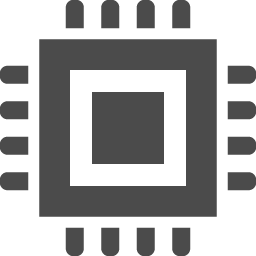
\includegraphics[height=11mm]{figs/assets/cpu.png}};
  \node[lbl, below=1pt of auicon] (aulab) {\textbf{Aurora} (static circuit)};
  \node[note, below=2pt of aulab] (aunote) {fixed R1CS; recompiles and re-audits on every change (update churn); transparent, so a post-quantum zero-knowledge proof is reachable};
  \node[below right=16mm and 16mm of rel] (vmicon) {
\includegraphics[height=11mm]{figs/assets/server.png}};
  \node[lbl, below=1pt of vmicon] (vmlab) {\textbf{zkVM} (RISC~Zero / SP1)};
  \node[note, below=2pt of vmlab] (vmnote) {one universal relation; a change is a guest-program edit, but the deployable post-quantum zero-knowledge proof is not reached on consumer hardware (Fig.~\ref{fig:dual-obstruction})};
  \draw[->] (rel) -- (auicon);
  \draw[->] (rel) -- (vmicon);
\end{tikzpicture}
\caption{One relation, two outer provers. The same BDEC verification relation is
proved \emph{either} by a static Aurora circuit (the BDEC baseline) \emph{or} by a
general-purpose zkVM (this thesis), and the two are alternatives: the zkVM does not
re-prove an Aurora proof. The figure locates the deployability wall: the static
Aurora circuit reaches a post-quantum zero-knowledge proof, whereas the zkVM does
not reach that proof on consumer hardware. The agility difference between the two
is a footprint distinction that this thesis measures and finds does not translate
into a per-proof wall-clock advantage.}
\label{fig:two-provers}
\end{figure}

\subsection{Contributions of This Thesis}

This thesis makes the following contributions.

\begin{enumerate}
  \item \textbf{A PLUM-instantiated BDEC artifact, validated in execute mode.} We express the verification predicate of the BDEC credential-generation (CreGen) relation as a guest program on RISC Zero, with PLUM in place of Loquat as the signature primitive, and we additionally run PLUM signature verification in isolation on SP1. We validate functional correctness in execute mode: at $\lambda=80$, BDEC CreGen executes both of its signature verifications to acceptance in $9.4\times10^{9}$ guest cycles, and we further realise the full ShowCre presentation relation as a $k+2$-verification guest and measure it in execute mode ($1.41\times10^{10}$ cycles at $k=1$ and $1.88\times10^{10}$ at $k=2$, confirming the additive cost model). To our knowledge this is the first realisation of PLUM-based BDEC components, both credential generation and presentation, in execute mode and the first standalone PLUM-verify prove-mode measurement, inside a general-purpose zkVM. % first-ness narrowed + prior art cited and distinguished in Section~\ref{sec:related} (S3 done 2026-06-06)

  \item \textbf{A deployable zero-knowledge proof not yet realised on consumer hardware.} Neither BDEC relation yet yields a zero-knowledge \emph{proof} on the target hardware: the CreGen succinct prove terminated in an internal-verifier anomaly distinct from a resource limit (an anomaly under diagnosis, Section~\ref{sec:evaluation}), and the ShowCre zero-knowledge wrap is bounded by the memory frontier of Section~\ref{sec:evaluation}. This is a measured negative result about the consumer-hardware frontier, \emph{not} an implementation gap in the artifact above.

  \item \textbf{A custom precompile suite as the instrument that makes the field-mismatch tax measurable.} We design and implement a Griffin-$\mathbb{F}_p^{192}$ precompile for the algebraic-hash primitive that the cost analysis of Section~\ref{sec:theoretical} identifies as the dominant tax-bearing operation, together with supporting big-integer arithmetic precompiles~\cite{cryptoeprint:2022/403}. We use it as the instrument that turns a non-terminating emulation into a finite standalone measurement, rather than treating it as a headline speedup: against the precompile-free path, which exhausts memory (OOM at $\approx$1m45s; Table~\ref{tab:plum-verify}) on the target hardware, the precompile reduces PLUM signature verification to a $32.5$-minute standalone prove on SP1 at $\lambda=80$. Introducing a custom AIR adds a trusted component to the verification path; the security statement is therefore \emph{conditional} on the constraint-level soundness of the Griffin AIR, which we carry as an open premise and discuss in Section~\ref{sec:security} (the conditional security-preservation theorem and premise~(T2)).

  \item \textbf{The bespoke algebraic-hash precompile is slower than a software SHA-3 control in this regime.} At matched $\lambda=80$, the Griffin-$\mathbb{F}_p^{192}$ precompile arm (Cell~2) does not outperform a PLUM arm that uses a software SHA-3 hasher and the existing big-integer precompile alone (Cell~3): it runs about $2.45\times$ slower in prove wall-clock ($32.5$ versus $13.3$ minutes), the metric on which deployment cost depends. We report this inversion as a substantive finding rather than a measurement artefact: in the deployed RISC~Zero/SP1 pipeline the cost of arithmetising a $199$-bit-field algebraic hash through a custom chip exceeds the cost of a SHA-class hash that the substrate already supports natively.

  \item \textbf{\emph{Update churn} as a measured evaluation dimension.} The rigidity of relation-specific circuits is a known structural property; we \emph{measure} its lifecycle cost. We define update churn quantitatively as the regeneration footprint incurred by a localised change to the verification relation: the set of compiled artefacts and proof-system parameters that must be regenerated and re-audited. We enumerate this footprint for both the static-circuit and zkVM regimes and use it to characterise a deployment-lifecycle trade-off that the current evaluation literature ignores.

  \item \textbf{A measurement of the consumer-hardware proving frontier.} On an Apple M5 Pro with $24$~GB of memory we report what the precompile-enabled zkVM regime can and cannot do at $\lambda=80$: PLUM signature verification proves in $32.5$ minutes on SP1, whereas BDEC CreGen runs correctly in execute mode but its default succinct proof terminated in an internal-verifier rejection: an anomaly under diagnosis (Section~\ref{sec:evaluation}), categorically distinct from a resource limit, on which no claim of this thesis rests. We report cycle counts, execute-mode wall-clock times, peak resident-set sizes, and (where proving completes) prove and verify times, with all parameters and procedures documented for reproducibility. The two regimes are compared directly on the update-churn dimension, which is independent of the runtime measurement.

  \item \textbf{A decision framework for practitioners.} On the basis of these measurements, we provide a framework that maps deployment-scenario parameters (policy-update frequency, hardware budget, anonymity-strength requirement) onto a regime recommendation, distinguishing the dimensions on which the comparison is currently conclusive (update churn) from those bounded by the consumer-hardware proving frontier.
\end{enumerate}

Taken together, these contributions answer a question the field has left open, namely whether a general-purpose zkVM is a viable substrate for post-quantum anonymous credentials on consumer hardware. The answer is \emph{not yet}, and the load-bearing reason is a single finding: on this hardware the BDEC proof one can afford to generate fails to be zero-knowledge, while the zero-knowledge wrap one can afford fails to be post-quantum. The first half is a measured resource bound; the second is a fact about the deployed toolchain, since the only wraps it exposes are pairing-based, so it holds independently of how favourable any timing number is and more memory does not remove it. This dual obstruction is the central finding of the thesis. The remaining contributions are the measurements that establish the surrounding cost picture, and two of them are findings precisely because they \emph{falsify} a natural prediction: a bespoke algebraic-hash precompile was expected to make verification fast, yet at matched $\lambda$ it runs slower than a software SHA-3 control (contribution~(4)); and a zkVM was expected to be more flexible than a static circuit, yet against the transparent baseline the recompile advantage is negligible (the update-churn dimension of contribution~(5)), becoming large only against a preprocessing baseline. The precompile suite (contribution~(3)) is what made these measurements finite; it serves as an instrument here rather than as a speedup in its own right, and no zero-knowledge BDEC proof was produced in this work. We report the implementation results as findings about where consumer-hardware proving holds and where it breaks, with contribution~(7) translating them into a deployment decision.

\subsection{Scope and Non-Goals}

This thesis is concerned with the practical deployability of PQ anonymous credentials on consumer hardware. We therefore make the following scope choices.

We focus on the BDEC framework~\cite{10.1007/978-981-96-0957-4_3} as the anonymous-credential construction, because (i) it is the leading symmetric-primitive-based PQ anonymous-credential system in the recent literature, (ii) its structure of two signature-verification predicates under a hidden user public key inside a zkSNARK is representative of a broad class of PQ-anon-cred designs, and (iii) its reliance on Aurora makes the static-circuit baseline well-defined and reproducible.

We focus on RISC Zero and SP1 as the zkVM substrates, because both expose application-defined precompiles, both target consumer hardware, and both serve as representative examples of the current generation of RISC-V-based zkVMs.

We do \emph{not} propose a new post-quantum signature scheme: we take PLUM as given and our contribution lies in how it is embedded into the broader credential system. We do \emph{not} propose new cryptographic assumptions: the security of the resulting system reduces to those already established for Loquat, PLUM, BDEC, RISC Zero, and SP1, together with a small number of premises that we state explicitly and carry as \emph{open} where they arise (the constraint-level soundness of the Griffin AIR, the existence of a PLUM signature-transcript simulator, and the quantum-random-oracle lifts), discharged in Section~\ref{sec:security} only as far as those references allow. We do \emph{not} claim that consumer-hardware PQ anonymous credentials are universally deployable today; rather, we quantify the cost frontier and identify the load-bearing pieces of the cost.

\subsection{Thesis Organisation}

The remainder of this thesis is structured as follows. Section~\ref{sec:related} surveys related work on post-quantum signatures, anonymous credentials, zkSNARKs, zkVMs, and precompile design. Section~\ref{sec:prelim} establishes the cryptographic primitives, signature schemes, zkSNARK and zkVM definitions, the BDEC construction, and the formal definition of update churn used throughout the thesis. Section~\ref{sec:theoretical} formalises the question we ask of each system regime and the comparative analysis we apply. Section~\ref{sec:system} describes the design and implementation of PLUM-in-BDEC in both the static-circuit and the zkVM regimes, including the precompile suite. Section~\ref{sec:evaluation} reports the empirical measurements on consumer hardware. Section~\ref{sec:discussion} interprets the measurements as a deployment-lifecycle decision framework. Section~\ref{sec:conclusion} concludes and identifies open problems.
